\documentclass[aspectratio=169,10pt]{beamer}

% ---------- Paquets ----------
\usefonttheme{professionalfonts}
\usepackage{fontspec}
\usepackage[french]{babel}
\usepackage{amsmath,amssymb}
\usepackage{booktabs}
\usepackage{array}
\usepackage{graphicx}
\usepackage{tikz}
\usetikzlibrary{arrows.meta,positioning,babel,shapes.geometric}
\usepackage{appendixnumberbeamer}
\graphicspath{{figures/}}

% ---------- Style ----------
\definecolor{bleu}{HTML}{1F4E79}
\definecolor{orange}{HTML}{E07B39}
\definecolor{vert}{HTML}{2E8B57}
\definecolor{rouge}{HTML}{C0392B}
\setbeamercolor{structure}{fg=bleu}
\setbeamercolor{frametitle}{fg=bleu}
\setbeamerfont{frametitle}{series=\bfseries,size=\Large}
\setbeamercolor{retenir}{bg=bleu!8,fg=black}
\setbeamercolor{block title}{bg=bleu,fg=white}
\setbeamercolor{block body}{bg=bleu!6}
\setbeamertemplate{blocks}[rounded]
\setbeamertemplate{navigation symbols}{}
\setbeamertemplate{itemize items}[circle]
\setbeamertemplate{section in toc}[sections numbered]
\setbeamertemplate{footline}{%
  \leavevmode\hbox to\paperwidth{\hspace{1.2em}\color{gray}\scriptsize\insertsectionhead\hfill
  \hyperlink{sommaire}{\color{bleu}\scriptsize$\hookleftarrow$ Sommaire}\hspace{1.5em}\insertframenumber{} / \inserttotalframenumber\hspace{1.2em}}\vspace{0.7em}}

% Encadré « À retenir »
\newcommand{\retenir}[1]{\vfill\begin{beamercolorbox}[sep=5pt,rounded=true]{retenir}\small\textbf{Élément clé :} #1\end{beamercolorbox}}
\newcommand{\Qdix}{Q\textsubscript{10}}
\newcommand{\CN}{{\NoAutoSpacing C:N}}

\title{Spatialisation du \Qdix{} pour les modèles de surface terrestre}
\subtitle{État d'avancement}
\author{Yassine Erraji \and William Peltier \and Simon Amar}
\date{Octobre 2026}

\begin{document}

% =====================================================================
\begin{frame}[plain]
  \titlepage
\end{frame}

\begin{frame}[label=sommaire]{Sommaire}
  \begin{columns}[t]
    \column{0.5\textwidth}\tableofcontents[sections={1-5}]
    \column{0.5\textwidth}\tableofcontents[sections={6-10}]
  \end{columns}
  \vfill
  {\small\color{gray}Chaque titre est cliquable ; le lien « Sommaire » en bas de chaque slide ramène ici.}
\end{frame}

% =====================================================================
\section{Démarche et hypothèses}

\begin{frame}{Le problème, en une slide}
  \begin{itemize}
    \item ORCHIDEE utilise un \Qdix{} \textbf{fixe} ($=2.0$) pour la décomposition de la matière organique du sol.
    \item \textbf{Objectif} : une carte de \Qdix{} qui fasse \textbf{mieux que 2.0 partout sur Terre}, pas seulement sur nos sites.
    \item \textbf{Point de départ} : Hacopian et al.\ (2026), régression linéaire $\Qdix \sim \text{MAT} + \text{MAP} + \text{pH}$ et carte mondiale.
    \item \textbf{Difficulté centrale} : généraliser à toute la planète à partir de \textbf{131 sites}, très concentrés géographiquement.
  \end{itemize}
  \retenir{toute la démarche consiste à juger chaque choix sur sa capacité à prédire \textbf{des régions jamais vues}.}
\end{frame}

\begin{frame}{Nos hypothèses de départ}
  \begin{enumerate}
    \item[H1] Le \Qdix{} varie avec le climat, le sol et la végétation, et cette variation se prédit à partir de cartes mondiales.
    \item[H2] Ajouter des variables (sol, humidité du sol, végétation) améliore la prédiction par rapport à MAT + MAP + pH.
    \item[H3] Des modèles d'apprentissage automatique plus flexibles battent les modèles linéaires.
    \item[H4] Des données synthétiques peuvent compenser le faible nombre de sites.
    \item[H5] Les coordonnées (latitude, longitude) portent une information utile.
    \item[H6] Le type de végétation (biome) est un prédicteur important.
  \end{enumerate}
  \retenir{\textbf{approche critique} : plusieurs de nos hypothèses ont été réfutées, et nous le montrons.}
\end{frame}

\begin{frame}{Notre démarche}
  \centering
  \begin{tikzpicture}[node distance=0.65cm and 0.75cm, boite/.style={draw=bleu, fill=bleu!8, rounded corners, align=center, text width=3.85cm, minimum height=1.35cm, font=\small, execute at begin node={\hyphenpenalty=10000}}, fl/.style={-{Stealth[length=2.2mm]}, bleu, thick}]
    \node[boite] (a) {\textbf{1. Données}\\131 sites};
    \node[boite, right=of a] (b) {\textbf{2. Enrichissement}\\sol, humidité, végétation};
    \node[boite, right=of b] (c) {\textbf{3. Protocole}\\validation croisée spatiale};
    \node[boite, below=of a] (d) {\textbf{4. Sélection}\\des variables (LASSO)};
    \node[boite, right=of d] (e) {\textbf{5. Comparaison}\\de 8 modèles};
    \node[boite, right=of e] (f) {\textbf{6. Extrapolation}\\vers la carte mondiale};
    \draw[fl] ([xshift=-0.9cm]a.north) to[out=115, in=65, looseness=1.6] node[above, font=\scriptsize, align=center, text=bleu] {recherche continue de nouvelles données\\(jeux de données privés, publications\dots)} ([xshift=0.9cm]a.north);
    \draw[fl] (a) -- (b);
    \draw[fl] (b) -- (c);
    \draw[fl] (c.south) -- ++(0,-0.32) -| (d.north);
    \draw[fl] (d) -- (e);
    \draw[fl] (e) -- (f);
  \end{tikzpicture}
\end{frame}

% =====================================================================
\section{Les données}

\begin{frame}{131 sites, très concentrés}
  \begin{columns}[c]
    \column{0.62\textwidth}
      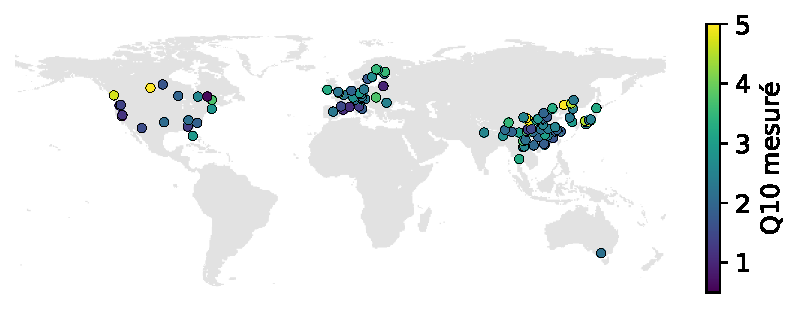
\includegraphics[width=\linewidth]{sites}
    \column{0.36\textwidth}
      \small
      \begin{itemize}
        \item 173 mesures de \Qdix{} microbien \textit{in situ}, 6 sources (Hacopian 2026 et compléments de l'équipe).
        \item Mesures d'un même point GPS \textbf{agrégées} : 131 sites.
        \item \textbf{99 \%} dans l'hémisphère Nord, \textbf{58 \%} en Asie de l'Est, \textbf{7} sous les tropiques.
        \item \textbf{Aucun} site en Afrique ni en Amérique du Sud.
      \end{itemize}
  \end{columns}
  \retenir{notre échantillon ne représente pas la planète : c'est la limite principale de tout le projet.}
\end{frame}

\begin{frame}{Un bruit local irréductible}
  \begin{columns}[c]
    \column{0.45\textwidth}
      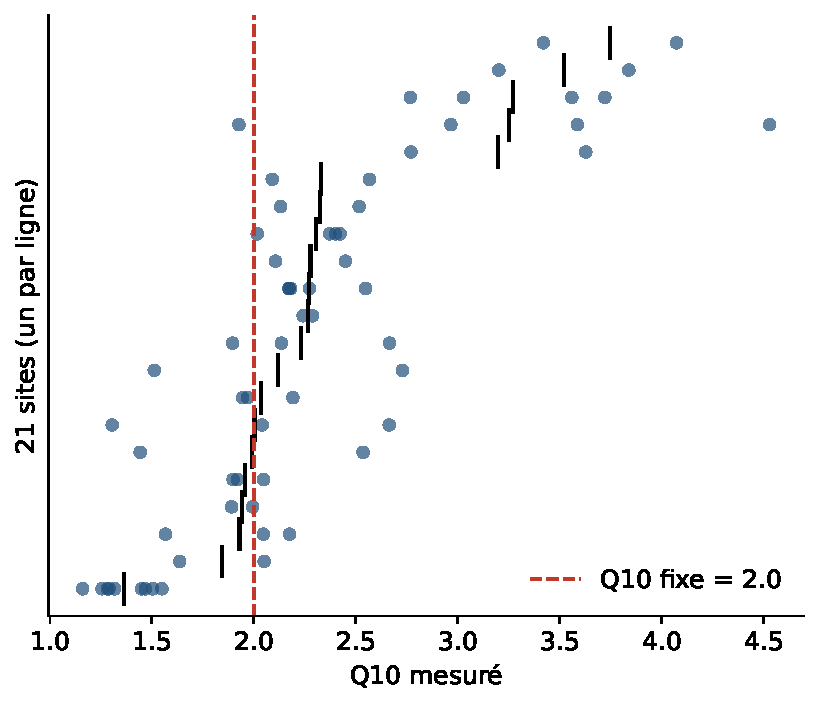
\includegraphics[width=\linewidth]{mesures_multiples}
    \column{0.53\textwidth}
      \small
      \begin{itemize}
        \item 21 sites portent plusieurs mesures (parcelles, peuplements, études) aux \textbf{mêmes variables} mais aux \Qdix{} différents.
        \item Écart-type au sein d'un site : $\hat\sigma_{\text{intra}} \approx 0.45$, contre $0.96$ au total.
        \item Aucune variable cartographiée ne peut expliquer cet écart : au mieux
        \[ R^2_{\max} \approx 1 - \frac{0.45^2}{0.96^2} \approx 0.78 . \]
        \item \textbf{Décision} : une ligne par site (\Qdix{} moyen), pour que chaque lieu pèse autant, comme sur une carte.
      \end{itemize}
  \end{columns}
  \retenir{une part de la variabilité du \Qdix{} est locale (essence, âge du peuplement, méthode) et restera inaccessible.}
\end{frame}

\begin{frame}{Variables explicatives : toutes disponibles en carte mondiale}
  \footnotesize
  \begin{tabular}{p{2.5cm}p{2.9cm}p{7.6cm}}
    \toprule
    Variable & Source & Définition \\
    \midrule
    MAT, MAP & ERA5-Land 1995--2024 & température de l'air à 2 m, précipitations annuelles \\
    SWC moyen & ERA5-Land 1995--2024 & humidité du sol 0--7 cm, moyenne annuelle \\
    SWC été relatif & ERA5-Land 1995--2024 & humidité des 3 mois les plus chauds / moyenne annuelle \\
    pH & SoilGrids 2.0 & 0--5 cm \\
    N, argile, sable, \CN{} & SoilGrids 2.0 & 5--15 cm, moyenne sur $\approx$ 15 km \\
    Végétation & RESOLVE 2017 & 3 classes : forêts extratropicales, forêts tropicales, végétation ouverte \\
    Latitude, longitude & --- & coordonnées du site \\
    \bottomrule
  \end{tabular}
  \vspace{0.3cm}
  \begin{itemize}
    \item \textbf{Validation} : en recalculant MAT, MAP, N et SWC été relatif, on retrouve les valeurs du jeu de l'équipe ($r$ de 0.98 à 0.996).
    \item \textbf{Écartées} : carbone organique (corrélé à 0.91 avec N) et température du sol (0.99 avec MAT), car redondants.
  \end{itemize}
\end{frame}

\begin{frame}{Ce que montrent les données}
  \begin{columns}[c]
    \column{0.5\textwidth}
      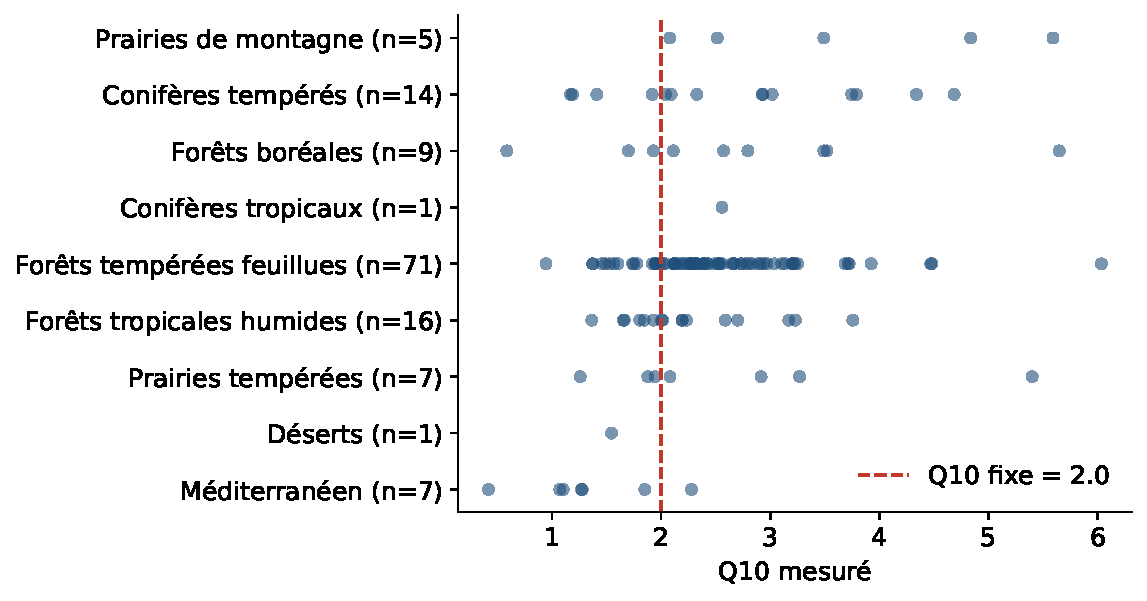
\includegraphics[width=\linewidth]{q10_biomes}
    \column{0.48\textwidth}
      \small
      \begin{itemize}
        \item Liens faibles pris isolément (Spearman) : MAT $-0.30$, N $+0.35$, longitude $+0.23$, SWC été relatif $+0.21$, MAP $-0.04$, pH $-0.12$.
        \item Comme chez Hacopian : \Qdix{} élevé en prairies de montagne (médiane 3.49), plus bas en forêts tropicales humides (2.10).
        \item \textbf{Nouveau} : les sites méditerranéens ont le \Qdix{} le plus bas (1.27) \textbf{et} l'été le plus sec (SWC été relatif 0.61, contre 0.94 à 1.11 ailleurs).
      \end{itemize}
  \end{columns}
  \retenir{un été sec semble freiner la réponse des microbes à la chaleur ; d'où l'intérêt de l'humidité du sol.}
\end{frame}

% =====================================================================
\section{Protocole d'évaluation}

\begin{frame}{Pourquoi une validation croisée \og spatiale \fg{} ?}
  \begin{columns}[c]
    \column{0.55\textwidth}
      \small
      \textbf{Validation croisée} : on découpe les sites en $K$ groupes, on entraîne sur $K-1$, on teste sur le dernier, et on tourne.
      \[ \text{RMSE}_{\text{CV}} = \frac{1}{K}\sum_{k=1}^{K} \sqrt{\frac{1}{|T_k|}\sum_{i\in T_k}\big(\Qdix_{,i}-\widehat{\Qdix}_{,i}\big)^2} \]
      \begin{itemize}
        \item Découpage \textbf{aléatoire} : un site de test a souvent un voisin presque identique à l'entraînement. Le score mesure en partie de la \textbf{mémoire}.
        \item Notre but est de prédire \textbf{des régions nouvelles} : on retire donc des zones géographiques entières.
      \end{itemize}
    \column{0.43\textwidth}
      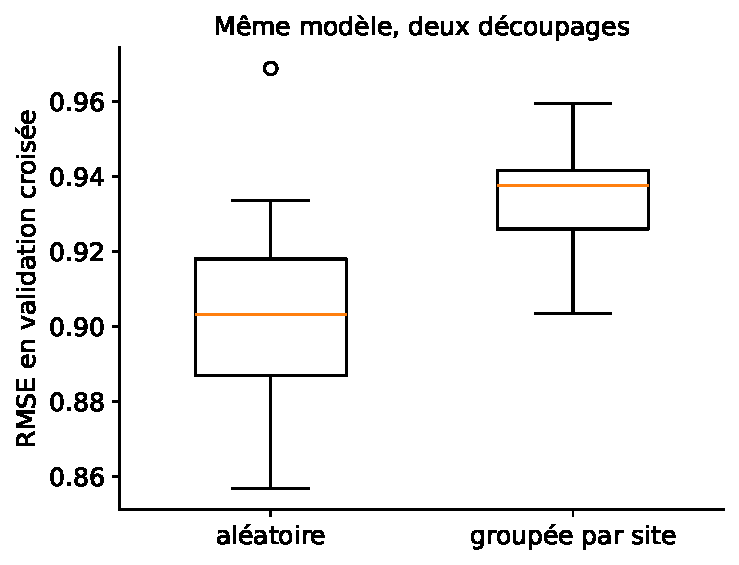
\includegraphics[width=\linewidth]{fuite_validation}
  \end{columns}
  \retenir{un découpage aléatoire surestime la qualité d'un modèle (0.90 contre 0.93 ici).}
\end{frame}

\begin{frame}{Quelle taille de zone ? Le semi-variogramme}
  \begin{columns}[c]
    \column{0.5\textwidth}
      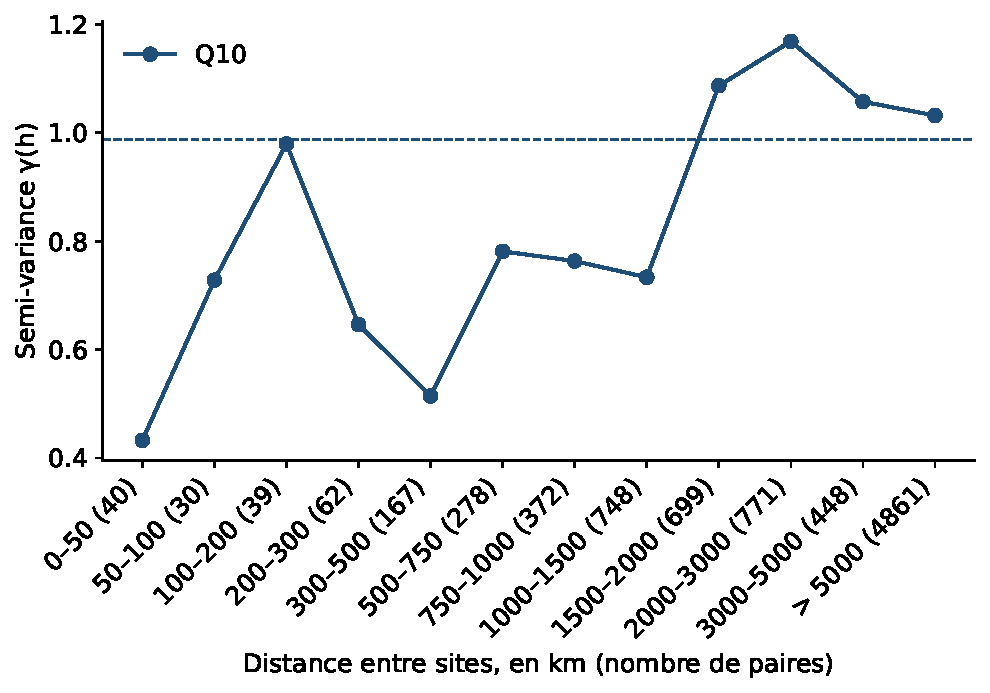
\includegraphics[width=\linewidth]{variogramme_q10}
      \centering\small\medskip
      $\gamma(h) = \tfrac12\,\mathbb{E}\big[(\Qdix(s)-\Qdix(s+h))^2\big]$\\[2pt]
      {\footnotesize moyenne sur toutes les paires de sites distants de $h$\par}
    \column{0.48\textwidth}
      \footnotesize
      \begin{itemize}
        \item Sous 50 km, $\gamma = 0.43$ : moins de la moitié de la variance (0.99, pointillés).
        \item Jusqu'à $\approx$ 1\,500 km, $\gamma$ reste sous la variance : les sites se ressemblent encore. Au-delà, palier (1.03 à 1.17).
        \item \textbf{Pic à 100--200 km (0.98)} : 39 paires seulement ; les 3 qui contiennent le site au \Qdix{} maximal (6.04) font la moitié de la somme. Sans ce site, $\gamma = 0.54$.
        \item \textbf{Palier au-dessus des pointillés} : la moyenne de $\gamma$ sur toutes les paires vaut exactement la variance. Les 57\,\% de paires à plus de 5\,000 km compensent donc les paires proches, sous la variance.
        \item \textbf{Choix} : zones de $10^\circ \times 10^\circ$ ($\approx$ 1\,100 km en latitude), 37 zones.
      \end{itemize}
  \end{columns}
  \retenir{les paires proches sont rares (1.3\,\% à moins de 200 km), d'où un début de courbe bruité. La portée ($\approx$ 1\,500 km) repose sur $\approx$ 700 paires par classe.}
\end{frame}

\begin{frame}{Le découpage retenu}
  \begin{columns}[c]
    \column{0.62\textwidth}
      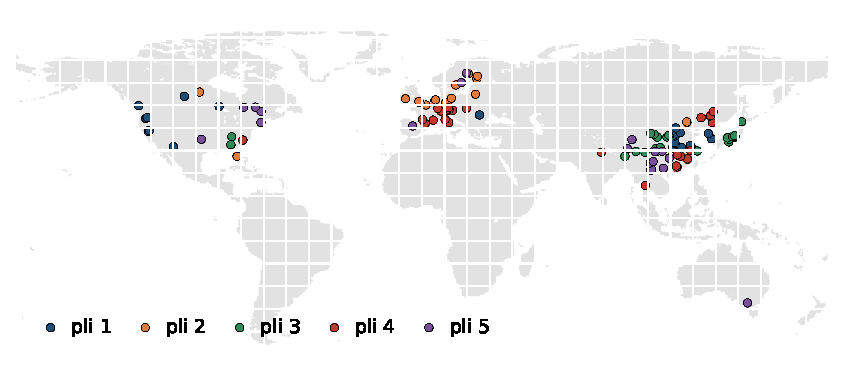
\includegraphics[width=\linewidth]{zones_spatiales}
    \column{0.36\textwidth}
      \small
      \begin{itemize}
        \item 5 plis : chaque pli retire $\approx$ 7 zones entières ($\approx$ 26 sites).
        \item Répété \textbf{20 fois} avec des découpages différents : 100 évaluations par modèle.
        \item \textbf{Mêmes découpages pour tous les modèles} : on peut les comparer pli par pli.
        \item Robustesse vérifiée avec des zones de $5^\circ$.
      \end{itemize}
  \end{columns}
\end{frame}

\begin{frame}{Cible et métriques}
  \small
  \textbf{Cible : $\log\Qdix$.} Si $R(T) = R_{\text{réf}}\;\Qdix^{(T-T_{\text{réf}})/10}$, alors $\ln R = \beta_0 + \beta_1 T$ et $\Qdix = e^{10\beta_1}$ :
  \begin{itemize}
    \item $\log\Qdix = 10\,\beta_1$ est directement la pente mesurée ;
    \item les prédictions $\widehat{\Qdix} = \exp(\widehat{\log\Qdix})$ restent positives, même en extrapolant ;
    \item la distribution devient plus symétrique (asymétrie $1.11 \to -0.68$). Une correction du biais de retransformation (Duan) a été testée : gain négligeable.
  \end{itemize}
  \textbf{Métriques, toujours sur l'échelle de \Qdix{}} :
  \[ \text{RMSE}=\sqrt{\tfrac1n\textstyle\sum_i(\Qdix_{,i}-\widehat{\Qdix}_{,i})^2},\quad \text{MAE}=\tfrac1n\textstyle\sum_i|\Qdix_{,i}-\widehat{\Qdix}_{,i}|,\quad R^2 = 1-\frac{\sum_i(\Qdix_{,i}-\widehat{\Qdix}_{,i})^2}{\sum_i(\Qdix_{,i}-\overline{\Qdix})^2} \]
  \[ \text{gain par rapport à 2.0} = 1 - \text{RMSE}_{\text{modèle}} / \text{RMSE}_{\Qdix=2.0} \]
\end{frame}

\begin{frame}{Comparer deux modèles honnêtement}
  \small
  \begin{itemize}
    \item L'erreur varie beaucoup d'un pli à l'autre selon les régions retirées : l'erreur standard calculée sur les plis d'un seul modèle vaut $\approx 0.12$, \textbf{plus que tous les écarts entre modèles}.
    \item On compare donc deux modèles $A$ et $B$ \textbf{sur les mêmes plis} : $d_k = \text{RMSE}^A_k - \text{RMSE}^B_k$.
    \item Les 100 plis ne sont pas indépendants (mêmes sites, entraînements qui se recouvrent). Correction de Nadeau et Bengio (2003) :
    \[ \widehat{\mathrm{SE}}(\bar d) = \sqrt{\Big(\frac{1}{K} + \frac{n_{\text{test}}}{n_{\text{entraînement}}}\Big)\, s_d^2}, \qquad K=100,\ \frac{n_{\text{test}}}{n_{\text{entr.}}}\approx\frac14 . \]
    \item \textbf{Règle de choix}, fixée à l'avance : le modèle \textbf{le plus simple} dont l'écart avec le meilleur reste sous une erreur standard. Ordre de simplicité : Elastic Net $<$ GAM $<$ SVR $<$ GP $<$ forêt aléatoire $<$ XGBoost, CatBoost, BART.
    \item \textbf{Second critère} : le comportement hors du domaine des données (pour la carte).
  \end{itemize}
  \retenir{pour qu'un modèle soit jugé meilleur qu'un autre, il lui faut de $\approx 0.02$ à $0.06$ de RMSE d'avance, selon les modèles comparés.}
\end{frame}

\begin{frame}{Les références à battre}
  \begin{columns}[c]
    \column{0.52\textwidth}
      \small
      \begin{tabular}{lcc}
        \toprule
        Référence & RMSE & Gain vs 2.0 \\
        \midrule
        $\Qdix = 2.0$ & 1.083 & --- \\
        moyenne des sites & 0.980 & 9.5 \% \\
        Hacopian, équation publiée & 0.994 & 8.3 \% \\
        Hacopian, réentraîné & \textbf{0.963} & \textbf{11.1 \%} \\
        \bottomrule
      \end{tabular}
      \vspace{0.2cm}

      {\footnotesize Équation publiée : $\Qdix = 0.109 - 0.0315\,\text{MAT} + 0.0002\,\text{MAP} + 0.411\,\text{pH}$.}
    \column{0.46\textwidth}
      \small
      \begin{itemize}
        \item \textbf{La moyenne bat déjà 2.0} ($-0.103 \pm 0.049$) : le \Qdix{} moyen de nos sites vaut 2.51.
        \item \textbf{L'équation publiée ne généralise pas} : elle bat 2.0 sur ses 70 sites d'origine (0.914 contre 1.118), mais fait moins bien sur les 61 autres (1.124 contre 1.106).
        \item Hacopian réentraîné ne se distingue pas de la moyenne ($-0.017 \pm 0.028$).
      \end{itemize}
  \end{columns}
  \retenir{battre 2.0 est facile ; battre la moyenne et Hacopian réentraîné est la vraie difficulté.}
\end{frame}

% =====================================================================
\section{Sélection des variables}

\begin{frame}{Premier tri : quelles variables ont leur place ?}
  \small
  Une variable n'entre dans le modèle que si elle remplit trois critères :
  \begin{enumerate}
    \item \textbf{disponible partout} : elle existe en carte mondiale (sinon, pas de carte possible) ;
    \item \textbf{plausible physiquement} : un moteur possible du \Qdix{}, pas un artefact d'échantillonnage ;
    \item \textbf{exploitable} : sans valeurs manquantes, et non redondante ($|\rho| < 0.8$).
  \end{enumerate}
  \vspace{0.2cm}
  \begin{itemize}
    \item \textbf{12 candidats} : MAT, log MAP, pH, log N, argile, sable, \CN{}, SWC moyen, SWC été relatif, végétation (3 classes), latitude, longitude.
    \item Un lien faible \textbf{pris isolément} ne suffit pas à exclure une variable : seul, MAP a un coefficient nul, mais $+0.12$ une fois MAT prise en compte (effet masqué).
    \item Coordonnées gardées (décision de l'équipe), avec une vigilance : elles décrivent surtout la géographie de nos sites.
  \end{itemize}
  \retenir{on ne tranche pas variable par variable : il faut une méthode de sélection rigoureuse.}
\end{frame}

\begin{frame}{La régularisation : principe}
  \begin{columns}[c]
    \column{0.6\textwidth}
      \small
      \textbf{Moindres carrés} : $\hat\beta = \arg\min_\beta \frac{1}{2n}\sum_i (y_i - x_i^\top\beta)^2$. Avec peu de sites et des variables corrélées, les coefficients sont \textbf{instables} (forte variance).

      \vspace{0.2cm}
      \textbf{Régulariser} : pénaliser la taille des coefficients (variables centrées-réduites) :
      \[ \hat\beta = \arg\min_\beta\ \tfrac{1}{2n}\textstyle\sum_i (y_i - x_i^\top\beta)^2 + \lambda\, P(\beta) \]
      \begin{itemize}
        \item \textbf{Ridge} : $P(\beta)=\|\beta\|_2^2=\sum_j\beta_j^2$, rétrécit tous les coefficients.
        \item \textbf{LASSO} : $P(\beta)=\|\beta\|_1=\sum_j|\beta_j|$, en met certains \textbf{exactement à zéro} : il sélectionne.
        \item \textbf{Elastic Net} : mélange des deux.
      \end{itemize}
      $\lambda$ règle le compromis biais / variance : il est choisi par validation croisée.
    \column{0.38\textwidth}
      \centering
      \begin{tikzpicture}[scale=0.85]
        \draw[->,gray] (-1.8,0) -- (2.4,0) node[right] {\small$\beta_1$};
        \draw[->,gray] (0,-1.8) -- (0,2.4) node[above] {\small$\beta_2$};
        \fill[bleu!20] (1.1,0) -- (0,1.1) -- (-1.1,0) -- (0,-1.1) -- cycle;
        \draw[bleu,thick] (1.1,0) -- (0,1.1) -- (-1.1,0) -- (0,-1.1) -- cycle;
        \draw[orange,thick,dashed] (0,0) circle (1.1);
        \draw[gray] (1.6,1.9) ellipse (1.0 and 0.5);
        \draw[gray] (1.6,1.9) ellipse (1.55 and 0.82);
        \fill (1.6,1.9) circle (1.5pt) node[above right] {\scriptsize$\hat\beta_{\text{MC}}$};
        \fill[bleu] (0,1.1) circle (2pt);
        \node[bleu,font=\scriptsize,align=right,anchor=east] (lab) at (-0.35,1.75) {LASSO : contact\\sur un coin ($\beta_1=0$)};
        \draw[bleu,->] (lab.east) -- (-0.05,1.17);
        \node[orange,font=\scriptsize] at (0.9,-1.4) {Ridge};
      \end{tikzpicture}
  \end{columns}
\end{frame}

\begin{frame}{LASSO : quelles variables survivent ?}
  \begin{columns}[c]
    \column{0.5\textwidth}
      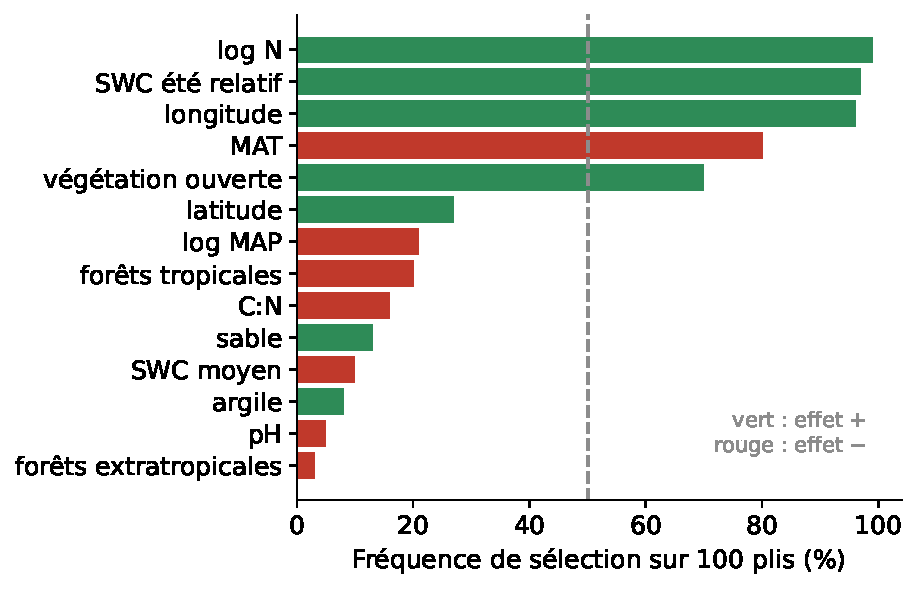
\includegraphics[width=\linewidth]{lasso_stabilite}
    \column{0.48\textwidth}
      \small
      \begin{itemize}
        \item LASSO refait sur chacun des 100 plis d'entraînement ; $\lambda$ choisi par validation croisée spatiale \textbf{interne}.
        \item Règle classique « d'un écart-type » : \textbf{aucune variable} dans 66 \% des plis (signal trop faible). On retient donc le $\lambda$ qui minimise l'erreur.
        \item \textbf{Noyau stable} (au moins 70 \% des plis, signe constant) : N ($+$), SWC été relatif ($+$), longitude ($+$), MAT ($-$), végétation ouverte ($+$).
        \item \textbf{Le pH}, central chez Hacopian, n'est retenu que dans 5 \% des plis.
      \end{itemize}
  \end{columns}
  \retenir{cinq variables portent un signal robuste ; c'est cohérent avec Hacopian pour MAT et la végétation, nouveau pour N et l'humidité estivale.}
\end{frame}

\begin{frame}{La végétation : un effet indécidable avec nos données}
  \begin{columns}[t]
    \column{0.48\textwidth}
      \small
      \textbf{Deux encodages testés} (régression Ridge, validation croisée spatiale) :

      \vspace{0.1cm}
      \begin{tabular}{lc}
        \toprule
        Végétation ajoutée & RMSE \\
        \midrule
        aucune & \textbf{0.934} \\
        typologie en 3 classes & 0.955 \\
        biomes (7 classes) & 0.969 \\
        \bottomrule
      \end{tabular}
      \begin{itemize}
        \item Le biome décrit la végétation \textbf{régionale potentielle}, pas celle de la parcelle (des plantations de pins y sont classées en « prairie »).
      \end{itemize}
    \column{0.5\textwidth}
      \small
      \textbf{Mais un test peu puissant} :
      \begin{itemize}
        \item Une fois le climat pris en compte, il reste un écart par biome dans le même sens que chez Hacopian (prairies de montagne $+0.90$, méditerranéen $-0.78$), non significatif ($p=0.10$).
        \item Simulation : si cet effet était réel, notre protocole ne le détecterait que \textbf{2 fois sur 3}.
        \item 47 \% des terres sont dans des biomes représentés par un site ou moins.
      \end{itemize}
  \end{columns}
  \retenir{« pas d'amélioration » ne veut pas dire « pas d'effet » : nos données excluent seulement un effet fort.}
\end{frame}

\begin{frame}{Ce que les variables n'expliquent pas}
  \begin{columns}[c]
    \column{0.55\textwidth}
      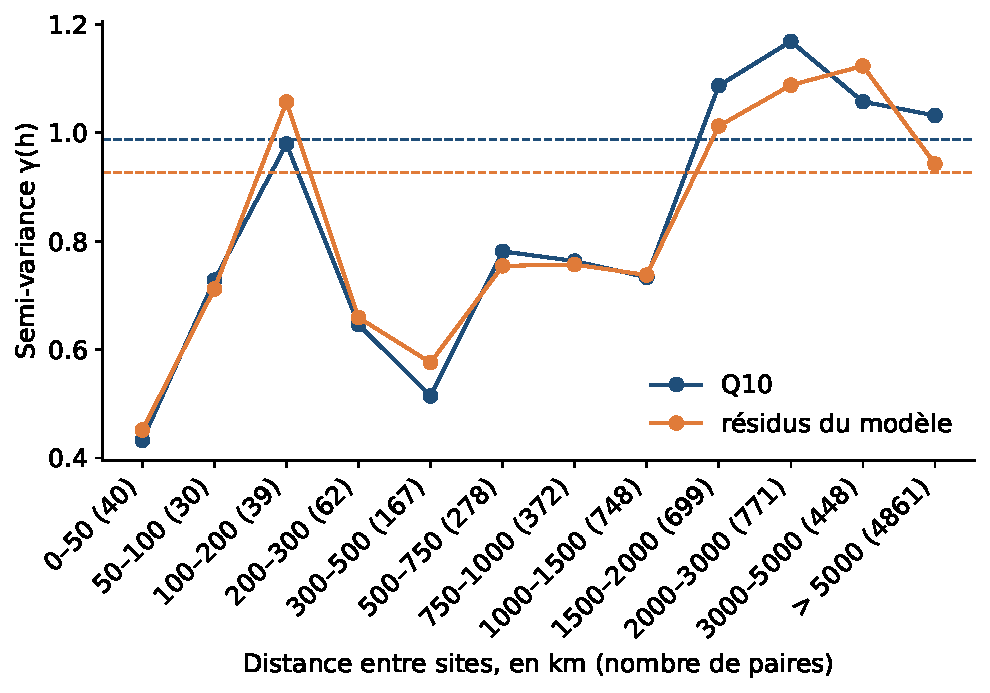
\includegraphics[width=\linewidth]{variogramme_residus}
    \column{0.43\textwidth}
      \small
      \begin{itemize}
        \item Semi-variogramme des \textbf{résidus} du modèle LASSO : presque identique à celui du \Qdix{}.
        \item La ressemblance entre sites voisins (jusqu'à $\approx$ 1\,500 km) \textbf{n'est pas expliquée} par le climat ni le sol.
        \item Elle pourrait venir de facteurs non cartographiés (communautés microbiennes, méthodes de mesure régionales\dots).
      \end{itemize}
  \end{columns}
  \retenir{une information spatiale reste à exploiter (krigeage des résidus), mais seulement près de nos sites.}
\end{frame}

% =====================================================================
\section{Modèles comparés}

\begin{frame}{Huit modèles, deux variantes, un protocole}
  \footnotesize
  \begin{tabular}{llll}
    \toprule
    Famille & Modèle & Idée & Hors du domaine \\
    \midrule
    Linéaire / additif & Elastic Net & droite pénalisée & prolonge la tendance \\
                       & GAM & somme de courbes lisses & prolonge les courbes \\
    Noyaux & SVR & similarité aux sites & revient vers une constante \\
           & Processus gaussien & krigeage dans l'espace des variables & revient vers la moyenne \\
    Arbres & Forêt aléatoire & moyenne d'arbres & constante \\
           & XGBoost, CatBoost & arbres ajoutés pas à pas & constante \\
           & BART & somme d'arbres bayésienne & constante \\
    \bottomrule
  \end{tabular}
  \vspace{0.3cm}
  \begin{itemize}
    \item \textbf{V1} : les 12 candidats. \textbf{V2} : sélection LASSO refaite dans chaque pli d'entraînement, puis le modèle.
    \item \textbf{Validation croisée imbriquée} : les plis externes évaluent ; des plis internes, eux aussi spatiaux, règlent les hyperparamètres.
    \item Tous les modèles apprennent $\log\Qdix$ sur exactement les mêmes plis.
  \end{itemize}
\end{frame}

\begin{frame}{Modèles linéaires et additifs}
  \small
  \textbf{Elastic Net} ($y=\log\Qdix$, variables centrées-réduites) :
  \[ \hat\beta = \arg\min_{\beta_0,\beta}\ \frac{1}{2n}\sum_{i=1}^n\big(y_i-\beta_0-x_i^\top\beta\big)^2 + \lambda\Big(\alpha\|\beta\|_1+\frac{1-\alpha}{2}\|\beta\|_2^2\Big) \]
  $\lambda$ et $\alpha$ (part du LASSO) choisis par validation croisée spatiale interne. Interprétable : un coefficient par variable.

  \vspace{0.3cm}
  \textbf{Modèle additif généralisé (GAM)} : chaque variable agit par une courbe lisse,
  \[ y_i = \beta_0 + \sum_{j} f_j(x_{ij}) + \varepsilon_i, \qquad f_j(x)=\sum_{k=1}^{8} b_{jk}\,B_k(x) \quad\text{(splines)} \]
  ajustée en minimisant $\sum_i (y_i-\hat y_i)^2 + \lambda \sum_j \int f_j''(x)^2\,dx$ : la pénalité de courbure empêche les courbes d'osciller. Capte des effets non linéaires (seuils) en restant lisible.
  \retenir{hors du domaine des données, ces modèles prolongent leur tendance : sur l'échelle de \Qdix{}, une droite en log devient une exponentielle.}
\end{frame}

\begin{frame}{Méthodes à noyau : SVR et processus gaussien}
  \small
  \textbf{SVR} : prédiction = somme pondérée de similarités aux sites, $f(x)=\sum_i \alpha_i\,k(x_i,x)+b$, avec $k(x,x')=e^{-\gamma\|x-x'\|^2}$.
  \[ \min_{f}\ \tfrac12\|f\|^2 + C\sum_i \max\big(0,\ |y_i-f(x_i)|-\epsilon\big) \]
  Les erreurs de moins de $\epsilon$ sont ignorées ; $C$, $\gamma$, $\epsilon$ réglés par validation croisée interne. Loin de tous les sites, $f(x)\to b$.

  \vspace{0.3cm}
  \textbf{Processus gaussien (GP)} : a priori $f\sim\mathcal{GP}(0,k)$, avec une échelle $\ell_j$ par variable :
  \[ k(x,x') = \sigma_f^2\exp\Big(-\tfrac12\sum_j\frac{(x_j-x'_j)^2}{\ell_j^2}\Big)+\sigma_n^2\,\delta_{xx'}, \qquad \hat f(x_*) = k_*^\top\,(K+\sigma_n^2 I)^{-1}\,y \]
  Hyperparamètres par maximum de vraisemblance marginale. Donne aussi une variance de prédiction.
  \retenir{le GP est l'analogue du \textbf{krigeage}, mais dans l'espace des variables explicatives plutôt que dans l'espace géographique.}
\end{frame}

\begin{frame}{Ensembles d'arbres}
  \small
  \textbf{Arbre de régression} : découpe l'espace des variables en rectangles, avec une valeur constante par rectangle.
  \begin{itemize}
    \item \textbf{Forêt aléatoire} : $\hat f(x)=\frac1B\sum_{b=1}^{B} T_b(x)$. Chaque arbre est entraîné sur un tirage avec remise des sites, avec un sous-ensemble aléatoire de variables à chaque coupure. La moyenne réduit la variance.
    \item \textbf{Boosting} (XGBoost, CatBoost) : arbres ajoutés un à un, chacun corrigeant les résidus des précédents,
    \[ F_m(x)=F_{m-1}(x)+\eta\,h_m(x), \qquad \min \sum_i \ell(y_i,F(x_i)) + \sum_m \Big(\gamma T_m + \tfrac12\lambda\|w_m\|^2\Big). \]
    \item \textbf{BART} : somme de petits arbres, avec des lois a priori qui limitent la contribution de chacun,
    \[ y = \sum_{m=1}^{M} g(x;\,T_m,\mu_m) + \varepsilon,\qquad \varepsilon\sim\mathcal N(0,\sigma^2), \]
    estimée par MCMC : prédiction moyenne et intervalles de crédibilité.
  \end{itemize}
  \retenir{flexibles et capables de capter des interactions, mais gourmands en données ; hors du domaine des données, leur réponse est plate.}
\end{frame}

% =====================================================================
\section{Résultats}

\begin{frame}{Seize configurations sur les mêmes plis}
  \begin{columns}[c]
    \column{0.66\textwidth}
      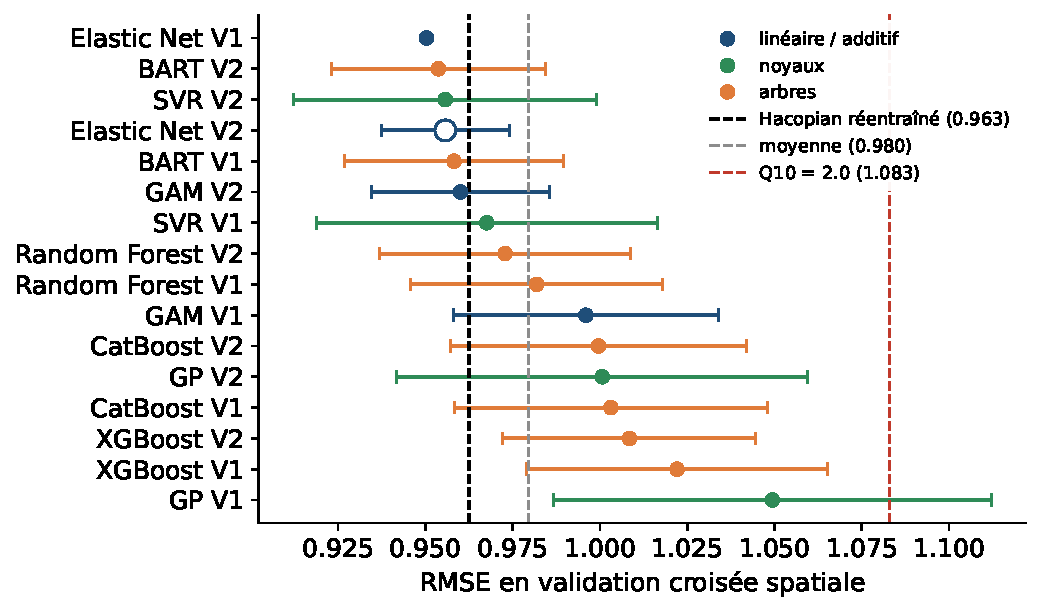
\includegraphics[width=0.97\linewidth]{comparaison_modeles}

      {\scriptsize\color{gray}Barres : $\pm$ une erreur standard de l'écart à la meilleure configuration.}
    \column{0.32\textwidth}
      \footnotesize
      \begin{itemize}
        \item Meilleure : Elastic Net V1 (0.950).
        \item \textbf{10 configurations équivalentes} (écart sous une erreur standard) : notre protocole ne peut pas les départager.
        \item Règle de choix : \textbf{Elastic Net V2} (0.956, $-11.7$ \% par rapport à 2.0), le plus simple.
        \item Boosting, CatBoost et GP font \textbf{moins bien que la moyenne}.
      \end{itemize}
  \end{columns}
  \retenir{avec 131 sites, la complexité ne paie pas : les modèles linéaires et additifs font au moins aussi bien.}
\end{frame}

\begin{frame}{Ce que vaut vraiment ce gain}
  \begin{columns}[t]
    \column{0.5\textwidth}
      \small
      \textbf{Elastic Net V2 face aux références} (écart $\pm$ erreur standard) :

      \vspace{0.1cm}
      \footnotesize
      \begin{tabular}{lcc}
        \toprule
        contre & écart & plis gagnés \\
        \midrule
        $\Qdix=2.0$ & $-0.127 \pm 0.056$ & 92 \% \\
        moyenne & $-0.024 \pm 0.059$ & 66 \% \\
        Hacopian réentraîné & $-0.007 \pm 0.062$ & 58 \% \\
        \bottomrule
      \end{tabular}
    \column{0.48\textwidth}
      \small
      \begin{itemize}
        \item Le gain sur 2.0 ($\approx$ 12 \%) est \textbf{net}.
        \item Mais \textbf{9.5 points} viennent du seul niveau moyen (2.51 sur nos sites).
        \item Le supplément apporté par les variables ($\approx$ 2 à 3 points) ne se distingue ni de la moyenne ni de Hacopian réentraîné.
        \item $R^2 \le 0.013$ pour tous les modèles en régions nouvelles.
      \end{itemize}
  \end{columns}
  \vspace{0.2cm}
  \small\textbf{Sélection en amont (V2 contre V1)} : elle aide ou est neutre pour tous les modèles (GAM : $-0.036 \pm 0.033$), sauf l'Elastic Net, qui sélectionne déjà lui-même.
  \retenir{battre 2.0 : oui. Mieux prédire les variations du \Qdix{} d'une région à l'autre : très peu, avec ces données.}
\end{frame}

\begin{frame}{Trois R², trois questions différentes}
  \small
  \[ R^2 = 1 - \frac{\sum_i(\Qdix_{,i}-\widehat{\Qdix}_{,i})^2}{\sum_i(\Qdix_{,i}-\overline{\Qdix})^2} \qquad \text{(0 pour la moyenne ; négatif si l'on fait moins bien qu'elle)} \]
  \footnotesize
  \begin{tabular}{>{\raggedright\arraybackslash}p{3.6cm}>{\raggedright\arraybackslash}p{4.4cm}>{\raggedright\arraybackslash}p{5.4cm}}
    \toprule
    R² calculé sur\dots & Question posée & Ce qu'il mesure \\
    \midrule
    les sites d'entraînement (\textbf{ajustement}) & le modèle décrit-il ses données ? & le \textbf{pouvoir explicatif}, celui des articles (Hacopian : $R^2 \approx 0.15$) \\
    des sites retirés au hasard (\textbf{VC aléatoire}) & prédit-il un site dont les voisins sont connus ? & l'interpolation \\
    des régions retirées (\textbf{VC spatiale}) & prédit-il une région jamais vue ? & le \textbf{pouvoir prédictif} utile pour la carte \\
    \bottomrule
  \end{tabular}
  \small
  \begin{itemize}
    \item \textbf{Plafond} : le bruit local entre mesures d'un même site limite le R² atteignable à $\approx 0.78$.
    \item \textbf{$r^2$} (carré de la corrélation entre observé et prédit) : mesure seulement si le modèle \textbf{classe} les sites dans le bon ordre, sans pénaliser un décalage ou une mauvaise échelle.
  \end{itemize}
  \retenir{un R² d'ajustement élevé ne garantit rien pour des régions nouvelles.}
\end{frame}

\begin{frame}{Pouvoir explicatif contre pouvoir prédictif}
  \begin{columns}[c]
    \column{0.55\textwidth}
      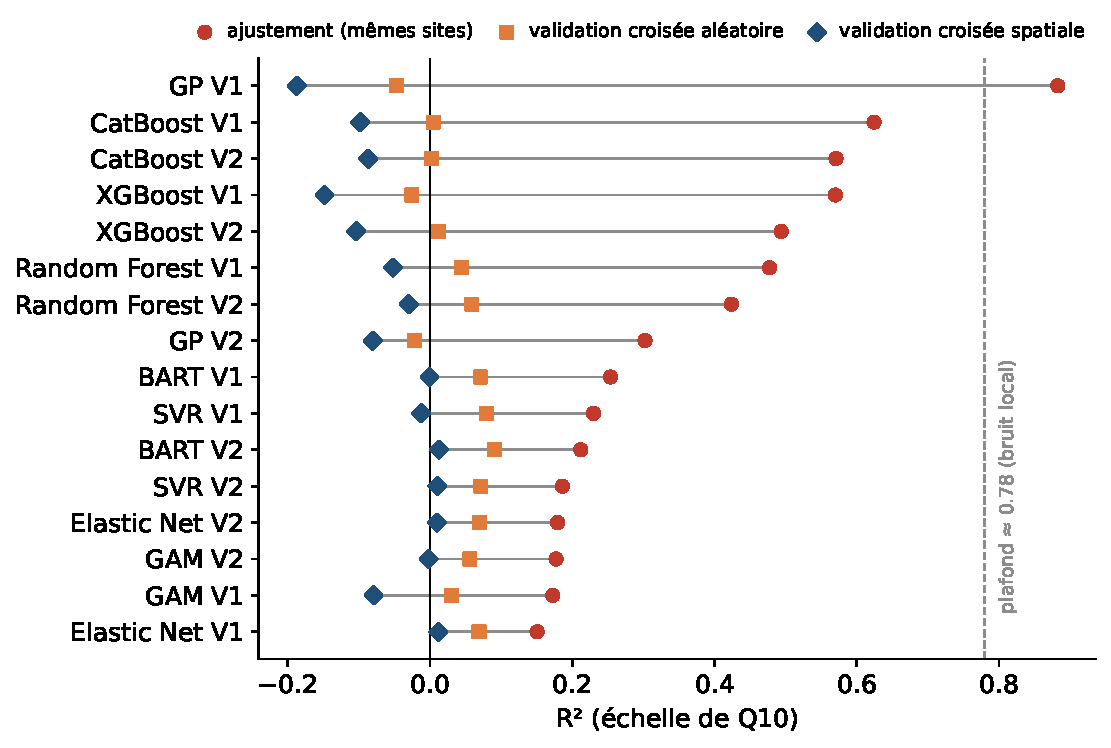
\includegraphics[width=\linewidth]{r2_trois}
    \column{0.43\textwidth}
      \small
      \begin{itemize}
        \item \textbf{Ajustement} : jusqu'à 0.88 (GP V1), \textbf{au-dessus du plafond} : le modèle apprend le bruit par cœur. Arbres : 0.42 à 0.62. Modèles retenus : 0.15 à 0.21.
        \item \textbf{VC aléatoire} : au mieux 0.09 (BART V2, Elastic Net $\approx$ 0.07).
        \item \textbf{VC spatiale} : au mieux 0.013 ; négatif pour les modèles flexibles.
        \item $r^2$ spatial jusqu'à 0.08 : les modèles classent un peu les sites, mais leurs prédictions restent trop proches de la moyenne.
      \end{itemize}
  \end{columns}
  \retenir{l'ordre s'inverse : plus un modèle explique ses propres sites, moins il prédit les régions nouvelles.}
\end{frame}

% =====================================================================
\section{Piste explorée : données synthétiques}

\begin{frame}{Augmenter les données avec une copule ?}
  \begin{columns}[t]
    \column{0.5\textwidth}
      \small
      \textbf{Théorème de Sklar} : toute loi jointe se sépare en marginales et en dépendance,
      \[ F(x_1,\dots,x_d) = C\big(F_1(x_1),\dots,F_d(x_d)\big). \]
      \textbf{Copule gaussienne} : $C_P(u)=\Phi_P\big(\Phi^{-1}(u_1),\dots,\Phi^{-1}(u_d)\big)$.

      \vspace{0.1cm}
      Génération : $z\sim\mathcal N(0,P)$, $u_j=\Phi(z_j)$, $x_j=\hat F_j^{-1}(u_j)$. La copule est ajustée sur les seuls sites d'entraînement de chaque pli.
    \column{0.48\textwidth}
      \small
      \begin{tabular}{lcc}
        \toprule
        & Ridge & Forêt \\
        \midrule
        sites réels & \textbf{0.933} & 1.000 \\
        $+$ 131 synthétiques & 0.954 & 0.988 \\
        $+$ 1\,000 synthétiques & 0.973 & 0.971 \\
        \bottomrule
      \end{tabular}
      \begin{itemize}
        \item Le Ridge se dégrade ; à pénalité égale, l'effet disparaît ($+0.004 \pm 0.012$).
        \item La forêt s'améliore un peu, sans dépasser une erreur standard : simple effet de régularisation.
      \end{itemize}
  \end{columns}
  \retenir{un générateur ajusté sur nos sites n'en sait pas plus qu'eux : aucune information nouvelle. Piste écartée.}
\end{frame}

% =====================================================================
\section{Vers la carte mondiale}

\begin{frame}{Une grille mondiale cohérente avec l'entraînement}
  \small
  \begin{itemize}
    \item Grille régulière de $0.5^\circ$ (de 90° N à 60° S) : \textbf{64\,745 cellules}, avec les mêmes sources et les mêmes définitions qu'à l'entraînement ; valeur d'une cellule = moyenne sur la cellule ($\approx$ 55 km).
    \item \textbf{Concordance aux sites} (valeur du site contre valeur de sa cellule) : corrélations de 0.92 (SWC moyen) à 0.99 (MAT, pH) ; 95 \% des sites ont la même classe de végétation que leur cellule.
  \end{itemize}
  \vspace{0.3cm}
  \textbf{Mais la grille sort largement de notre domaine :}
  \begin{itemize}
    \item MAT de nos sites : $-5.2$ à $24.5$ °C ; sur la grille : $-22.2$ à $33.5$ °C. MAT seule est hors de la plage sur \textbf{38 \%} des terres.
    \item \textbf{64 \%} des terres ont au moins une variable hors de la plage observée.
  \end{itemize}
  \retenir{passer du site à la maille de 0.5° change peu les variables ; le vrai problème est l'extrapolation.}
\end{frame}

\begin{frame}{Où le modèle extrapole-t-il ? L'aire d'applicabilité}
  \begin{columns}[c]
    \column{0.6\textwidth}
      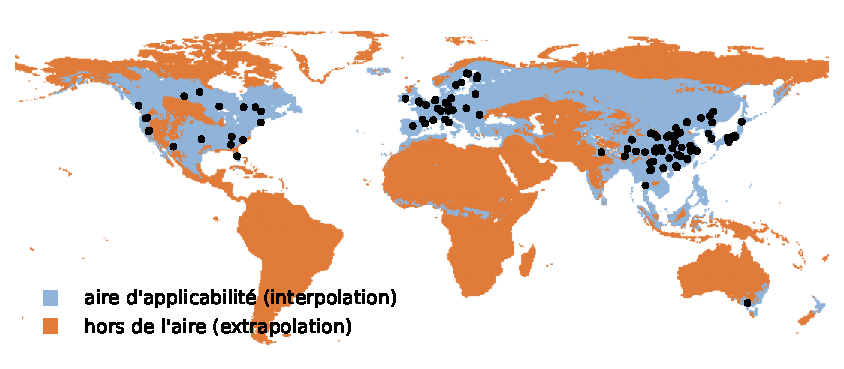
\includegraphics[width=\linewidth]{aire_applicabilite}
    \column{0.38\textwidth}
      \small
      Meyer et Pebesma (2021), dans l'espace centré-réduit des 6 variables du modèle retenu :
      \[ \mathrm{DI}(x) = \frac{\min_i \|z(x)-z_i\|}{\bar d} \]
      ($\bar d$ : distance moyenne entre sites). Seuil : $Q_3 + 1.5\,\mathrm{IQR}$ des DI des sites, calculés par rapport aux autres zones.
      \begin{itemize}
        \item \textbf{36 \% des terres} sont dans l'aire d'applicabilité.
      \end{itemize}
  \end{columns}
  \retenir{l'Amérique du Sud, l'Afrique, l'Australie intérieure, l'Arctique et la Sibérie sont des extrapolations.}
\end{frame}

\begin{frame}{Comment les modèles extrapolent}
  \centering
  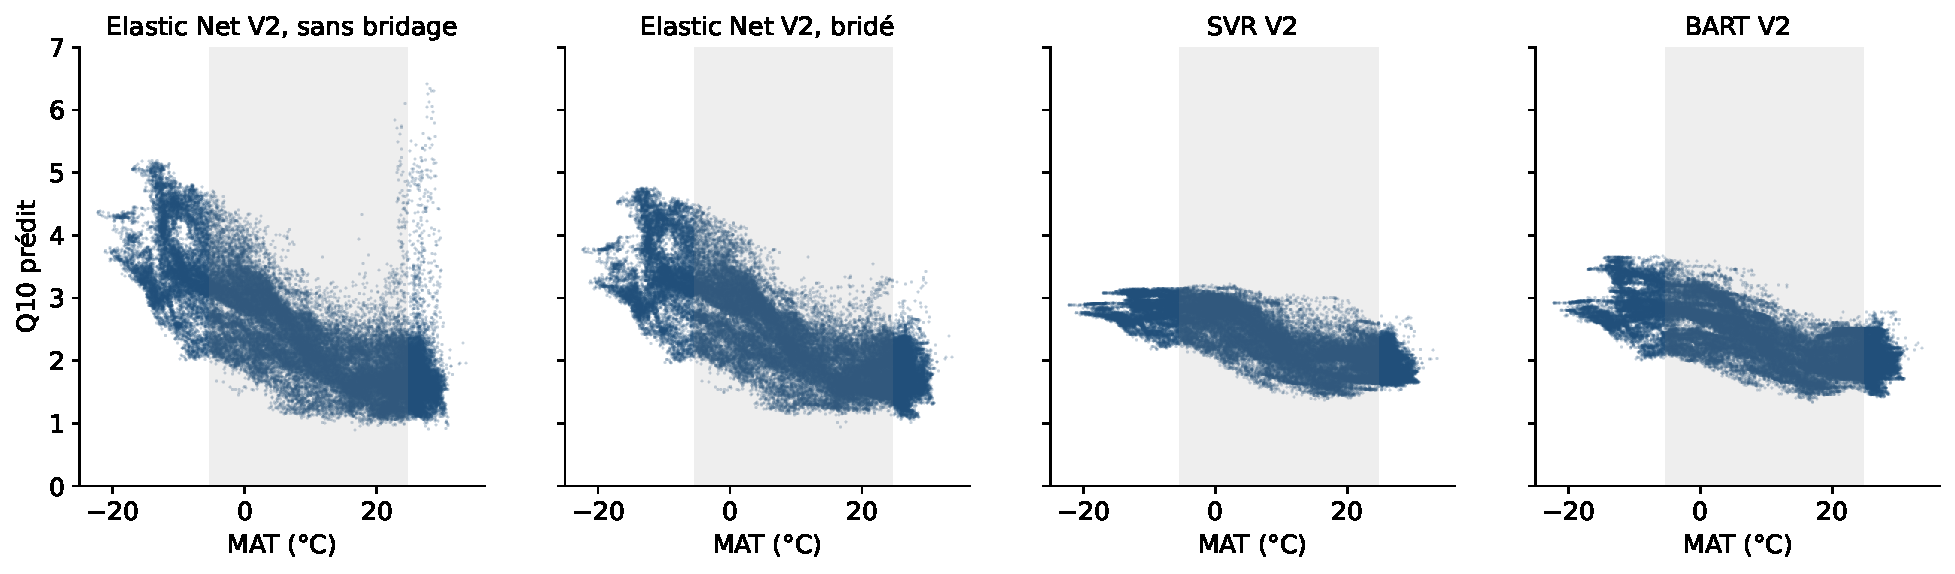
\includegraphics[width=\linewidth]{formes_reponse}
  \small
  \begin{itemize}
    \item Zone grisée : plage de MAT de nos sites. L'Elastic Net prolonge la tendance (\Qdix{} plus élevé au froid) ; SVR et BART s'aplatissent.
    \item \textbf{Artefact} : pics jusqu'à 6.4 au Sahara. « SWC été relatif » y divise deux humidités quasi nulles ($\approx$ 0.001 m³/m³) et devient du bruit.
    \item \textbf{Correction : le bridage} $\tilde x_j=\min\big(\max(x_j,\min_i x_{ij}),\max_i x_{ij}\big)$. Il supprime l'artefact (maximum au Sahara : 6.40 → 2.68) et améliore même légèrement la validation croisée (0.956 → 0.950).
  \end{itemize}
\end{frame}

\begin{frame}{Là où le choix du modèle compte}
  \centering
  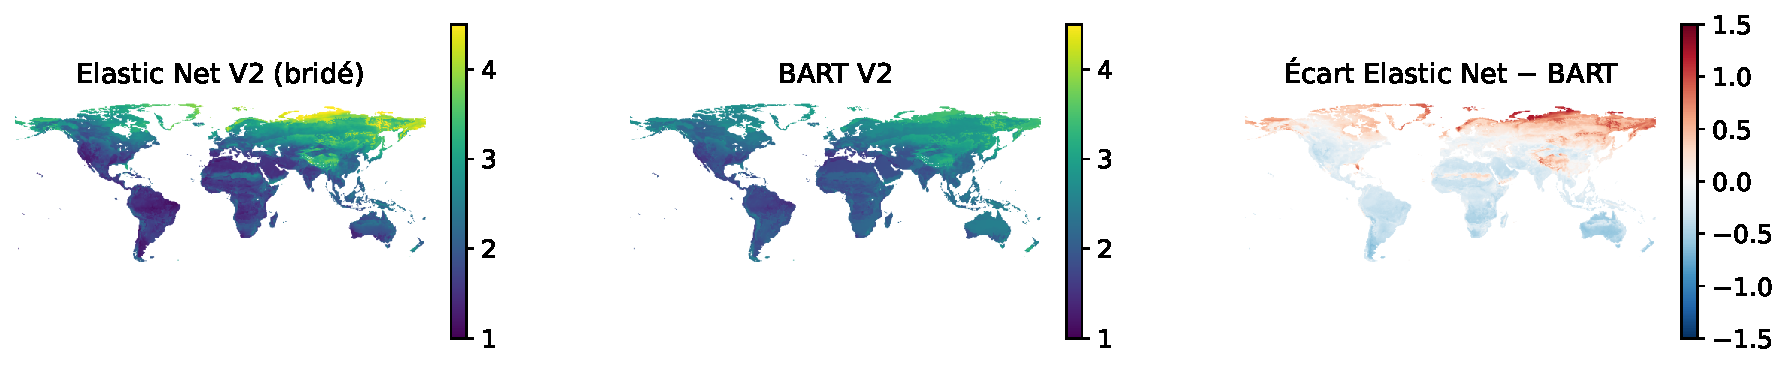
\includegraphics[width=\linewidth]{cartes_modeles}
  \small
  \begin{columns}[t]
    \column{0.5\textwidth}
      \begin{itemize}
        \item \textbf{Dans l'aire d'applicabilité}, les modèles s'accordent (\Qdix{} moyen $\approx$ 2.4).
        \item \textbf{\Qdix{} moyen mondial} : 2.1 à 2.2 selon le modèle, proche de 2.0.
      \end{itemize}
    \column{0.48\textwidth}
      \begin{itemize}
        \item \textbf{Régions froides} (10 \% des terres, aucun site) : Elastic Net 3.40, BART 2.92, SVR 2.82, Hacopian 2.97.
      \end{itemize}
  \end{columns}
  \retenir{la carte apporte surtout une \textbf{répartition} du \Qdix{} ; l'incertitude est maximale là où se trouve le permafrost.}
\end{frame}

% =====================================================================
\section{Bilan critique et suite}\label{sec:bilan}

\begin{frame}{Nos hypothèses, confrontées aux résultats}
  \small
  \begin{tabular}{p{0.42\textwidth}p{0.5\textwidth}}
    \toprule
    Hypothèse & Verdict \\
    \midrule
    H1 --- \Qdix{} prévisible depuis des cartes & \textbf{en partie} : signal robuste mais faible ($R^2\approx0$ en régions nouvelles) \\
    H2 --- plus de variables aident & \textbf{en partie} : N et SWC été relatif entrent dans le noyau ; le pH n'y survit pas \\
    H3 --- le ML flexible bat le linéaire & \textcolor{rouge}{\textbf{non}} : linéaire et additif en tête ; boosting et GP sur-apprennent (R² d'ajustement jusqu'à 0.88, R² spatial négatif) \\
    H4 --- les données synthétiques compensent & \textcolor{rouge}{\textbf{non}} : aucune information nouvelle \\
    H5 --- les coordonnées sont utiles & \textbf{oui pour la longitude} (effet Asie de l'Est) ; origine à éclaircir \\
    H6 --- le biome est un bon prédicteur & \textbf{indécidable} avec nos données (test peu puissant) \\
    \bottomrule
  \end{tabular}
\end{frame}

\begin{frame}{Ce que nous avons appris}
  \begin{enumerate}
    \item \textbf{Les données sont le facteur limitant} : 131 sites concentrés sur trois régions ; le modèle extrapole sur 64 \% des terres.
    \item \textbf{Battre 2.0 est facile, mais surtout par le niveau moyen.} Les variables n'ajoutent que 2 à 3 points, ce qui ne se distingue ni de la moyenne ni de Hacopian réentraîné.
    \item \textbf{Les modèles simples gagnent} : les plus flexibles expliquent jusqu'à 88 \% de la variance de leurs propres sites, mais rien dans des régions nouvelles.
    \item \textbf{Signaux robustes} : azote, sécheresse estivale, MAT, effet Asie de l'Est, végétation ouverte.
    \item \textbf{L'incertitude de la carte vient de l'extrapolation}, et elle est maximale dans les régions froides.
  \end{enumerate}
\end{frame}

\begin{frame}{Limites de notre approche}
  \small
  \begin{itemize}
    \item \textbf{Représentativité} : aucun site plus froid que $-5.2$ °C, aucun en Afrique ni en Amérique du Sud. Le \Qdix{} moyen de nos sites (2.51) n'est pas forcément celui de la planète.
    \item \textbf{Hétérogénéité des mesures} : méthodes de séparation des respirations, plages de température et durées différentes d'une étude à l'autre. Aucun biais net par source, mais un bruit qui s'ajoute.
    \item \textbf{Végétation} : le biome décrit la végétation potentielle, pas celle de la parcelle.
    \item \textbf{Échelle} : un \Qdix{} de parcelle prédit à l'échelle d'une maille de 0.5° (concordance des variables vérifiée, mais le \Qdix{} lui-même peut dépendre de l'échelle).
    \item \textbf{Puissance statistique} : avec 131 sites, des effets modérés (biome, interactions) restent indétectables.
    \item \textbf{Longitude} : son effet peut refléter des pratiques de mesure régionales autant qu'un vrai signal ; il reste figé si le climat change.
  \end{itemize}
\end{frame}

\begin{frame}{Proposition : un niveau de confiance et une valeur de repli}
  \begin{columns}[c]
    \column{0.6\textwidth}
      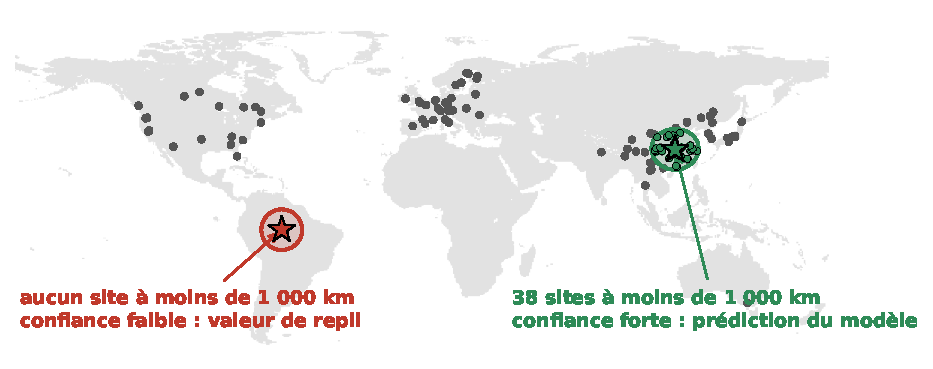
\includegraphics[width=\linewidth]{confiance}
    \column{0.38\textwidth}
      \small
      \begin{itemize}
        \item \textbf{Confiance} : $c(x)=\min\big(1,\,n_r(x)/n^*\big)$, où $n_r(x)$ est le nombre de sites à moins de $r\approx 1\,000$ km (portée du semi-variogramme).
        \item \textbf{Règle} : prédiction du modèle si $c(x)\ge\alpha$ ; sinon \textbf{valeur de repli} : 2.0, ou une valeur propre à la zone.
        \item \textbf{Sans saut} : $c\,\hat f + (1-c)\,\Qdix^{\text{repli}}$.
        \item \textbf{Aujourd'hui} : 30 \% des terres ont au moins un site à moins de 1\,000 km ; 13 \% en ont au moins cinq.
      \end{itemize}
  \end{columns}
  \retenir{la carte prédirait là où elle dispose d'informations (en combinant cette confiance avec l'aire d'applicabilité), et reviendrait à une valeur prudente ailleurs.}
\end{frame}

\begin{frame}{Pistes à explorer}
  \small
  \begin{itemize}
    \item \textbf{Ajouter des sites là où ils manquent}, en priorité les régions froides et tropicales : c'est le levier le plus puissant.
    \item \textbf{Végétation réelle} : occupation du sol satellitaire (MODIS) ou PFT d'ORCHIDEE à la place du biome.
    \item \textbf{Modèle hiérarchique} : effet aléatoire par classe de végétation, qui rétrécit les effets des petits groupes au lieu de les ignorer.
    \item \textbf{Krigeage des résidus} : exploiter la structure spatiale non expliquée, près des sites.
    \item \textbf{Carte d'incertitude} : intervalles de crédibilité du BART, combinés à l'aire d'applicabilité.
    \item \textbf{\Qdix{} dynamique} : une relation $\Qdix = f(\text{climat})$ utilisable dans les scénarios.
    \item \textbf{Au-delà du \Qdix{}} : Hacopian montre que le modèle MMRT décrit mieux la réponse à la température.
  \end{itemize}
\end{frame}

% =====================================================================
\appendix
\section{Annexes}

\begin{frame}{Annexe --- Les 16 configurations}
  \small
  \begin{columns}[t]
    \column{0.48\textwidth}
      \begin{tabular}{lcc}
        \toprule
        Configuration & RMSE & Gain vs 2.0 \\
        \midrule
        Elastic Net V1 & 0.950 & 12.2 \% \\
        BART V2 & 0.954 & 11.9 \% \\
        SVR V2 & 0.956 & 11.7 \% \\
        \textbf{Elastic Net V2} & \textbf{0.956} & \textbf{11.7 \%} \\
        BART V1 & 0.958 & 11.5 \% \\
        GAM V2 & 0.960 & 11.3 \% \\
        \textit{Hacopian réentraîné} & \textit{0.963} & \textit{11.1 \%} \\
        SVR V1 & 0.968 & 10.6 \% \\
        Forêt aléatoire V2 & 0.973 & 10.2 \% \\
        \textit{moyenne} & \textit{0.980} & \textit{9.5 \%} \\
        \bottomrule
      \end{tabular}
    \column{0.48\textwidth}
      \begin{tabular}{lcc}
        \toprule
        Configuration & RMSE & Gain vs 2.0 \\
        \midrule
        Forêt aléatoire V1 & 0.982 & 9.3 \% \\
        \textit{Hacopian publié} & \textit{0.994} & \textit{8.3 \%} \\
        GAM V1 & 0.996 & 8.0 \% \\
        CatBoost V2 & 1.000 & 7.7 \% \\
        GP V2 & 1.001 & 7.6 \% \\
        CatBoost V1 & 1.003 & 7.4 \% \\
        XGBoost V2 & 1.008 & 6.9 \% \\
        XGBoost V1 & 1.022 & 5.6 \% \\
        GP V1 & 1.049 & 3.1 \% \\
        \textit{$\Qdix=2.0$} & \textit{1.083} & --- \\
        \bottomrule
      \end{tabular}
  \end{columns}
\end{frame}

\begin{frame}{Annexe --- Réglages des modèles}
  \footnotesize
  \begin{tabular}{lll}
    \toprule
    Modèle & Réglés par validation croisée spatiale interne & Autres choix \\
    \midrule
    Elastic Net & $\lambda$ (10 valeurs), part du LASSO $\alpha\in\{0.1,0.5,0.9\}$ & --- \\
    GAM & pénalité de courbure (5 valeurs) & 8 splines par variable \\
    SVR & $C$, $\gamma$, $\epsilon$ (36 combinaisons) & noyau gaussien \\
    GP & par vraisemblance marginale & une échelle par variable \\
    Forêt aléatoire & variables par coupure, taille des feuilles & 200 arbres \\
    XGBoost & profondeur, pénalité $\lambda$ & 300 arbres, $\eta=0.03$ \\
    CatBoost & profondeur, pénalité $\ell_2$ & 300 arbres, $\eta=0.05$ \\
    BART & aucun (lois a priori par défaut) & 500 tirages MCMC conservés \\
    \bottomrule
  \end{tabular}
  \vspace{0.3cm}

  Grilles volontairement petites : 131 sites, 100 plis externes, plis internes eux aussi spatiaux.
\end{frame}

\begin{frame}{Annexe --- Sélection LASSO sur 100 plis}
  \small
  \begin{tabular}{lcc@{\hspace{1.2cm}}lcc}
    \toprule
    Variable & Fréquence & Signe & Variable & Fréquence & Signe \\
    \midrule
    log N & 99 \% & $+$ & \CN{} & 16 \% & $-$ \\
    SWC été relatif & 97 \% & $+$ & sable & 13 \% & $+$ \\
    longitude & 96 \% & $+$ & SWC moyen & 10 \% & mixte \\
    MAT & 80 \% & $-$ & argile & 8 \% & mixte \\
    végétation ouverte & 70 \% & $+$ & pH & 5 \% & $-$ \\
    latitude & 27 \% & $+$ & forêts extratropicales & 3 \% & $-$ \\
    log MAP & 21 \% & $-$ & & & \\
    forêts tropicales & 20 \% & $-$ & & & \\
    \bottomrule
  \end{tabular}
  \vspace{0.3cm}

  LASSO avec la pénalité qui minimise l'erreur de la validation croisée spatiale interne ; médiane de 5 variables retenues par pli. Performance : RMSE 0.954 (Ridge sur toutes les variables : 0.953).
\end{frame}

\end{document}
